\chapter{Implementación del sistema.}
\label{cap: capitulo_5}

A lo largo de este capítulo vamos a explicar cómo hemos llevado a cabo el proceso de implementación del sistema, partiendo del diseño especificado en las páginas anteriores.

Todos los bloques se han implantado con una filosofía similar, teniendo en cuenta que nos dirigimos a un sistema empotrado, de prestaciones limitadas, y donde la seguridad y el tiempo de respuesta son cruciales.

Debemos tener también en cuenta que el servicio podrá ser utilizado por varios usuarios a la vez ---incluso varios componentes--- y el planificador, si bien no requiere características de tiempo-real estricto, es necesario que responda adecuadamente a los tiempos marcados por la partitura.

En el demonio, nuestra máxima prioridad será la eficiencia, mientras que en la interfaz \textit{web} nos centraremos en la accesibilidad.

\section{Planificación}

\section{Servicio del reproductor}

Este bloque compone el \textit{back-end} del sistema. Comprende una gran cantidad de elementos técnicos y hace uso de numerosas funciones del sistema operativo. Vamos a escribirlo casi por completo en lenguaje C, por las siguientes razones:

\begin{enumerate}
	\item Alta calidad y eficiencia.
	\item Cercanía al \textit{hardware}.
	\item Capacidad para hacer llamadas al sistema Linux.
	\item Posibilidad de acceder al código ensamblador para hacer optimizaciones.
\end{enumerate}

Aunque todos los ejecutables se van a compilar desde código \textit{C}, haremos uso de \textit{shell-scripts} y un \textit{Makefile} que nos permitirá compilar fácilmente las fuentes e instalar los ejecutables.

En ciertos componentes, necesitaremos hacer \textbf{prototipos} para estudiar su funcionamiento y realizar pruebas de concepto, antes de implantarlos definitivamente. Esto lo haremos en Python, un lenguaje interpretado y de programación más ágil que C.

En resumen, utilizaremos el siguiente procedimiento con los componentes más complejos, que así lo requieran:

\smallskip

\begin{figure}[H]
	\noindent \begin{centering}
		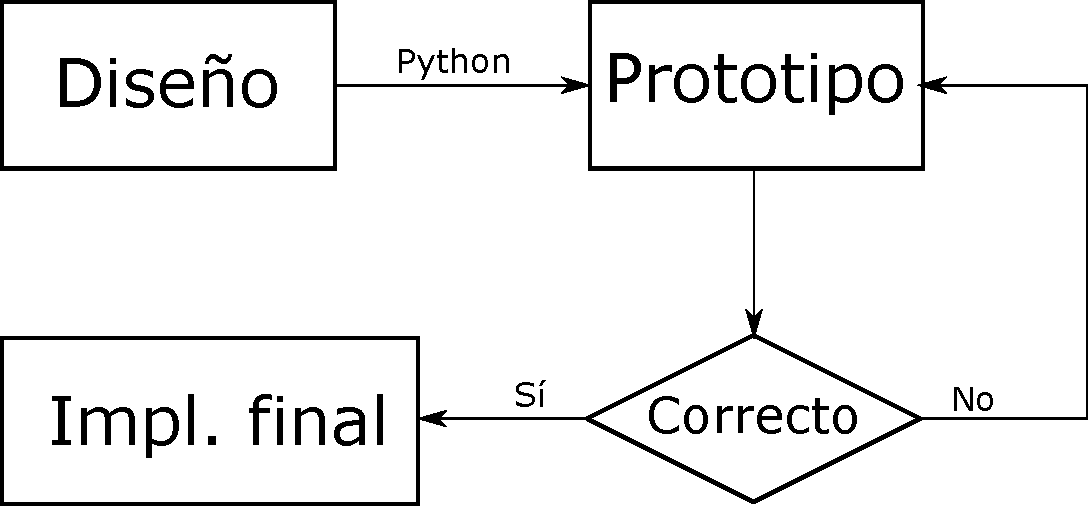
\includegraphics[width=\linewidth/2]{capitulo5/prototipado}
		\par\end{centering}
	\smallskip
	\caption{\label{fig:prototipado} Esquema de prototipado.}
\end{figure} 

\smallskip

El código hace uso de los siguientes componentes externos:

\begin{enumerate}
	\item Biblioteca estándar de C \cite{cplusplus}.
	\item Interfaz \acrshort{POSIX} \cite{wiki_posix}.
	\item Llamadas al sistema Linux \cite{manpages}.
	\item Sistema de archivos especial \textit{GPIOFS} \cite{gpiofs}.
	\item Biblioteca \textit{WiringPi} (solo para el modo Ingeniería) \cite{wiringpi}.
	\item Biblioteca estándar de Python (para los prototipos) \cite{python}.
\end{enumerate}

\subsection{Descodificador de MIDI}

Este fue el primer módulo a implementar. Estudiado el análisis, el diseño es sencillo por la independencia entre eventos. Sin embargo, la implementación presentaba una complejidad notable, sobre todo porque no hay un carácter separador entre eventos, y tanto los meta-eventos como las marcas de duración tienen longitud variable.

Como ya indicamos en la sección \ref{sec:fmto_midi}, el protocolo \acrshort{MIDI} especifica que los valores numéricos se indican en \textit{big-endian}. Como el procesador del \textit{Raspberry} funciona en \textit{little-endian}, hay que intercambiar los \textit{bytes} de los números que ocupen más de un \textit{byte}. La figuras siguientes ilustran este problema:

\smallskip

\begin{figure}[H]
	\noindent \begin{centering}
		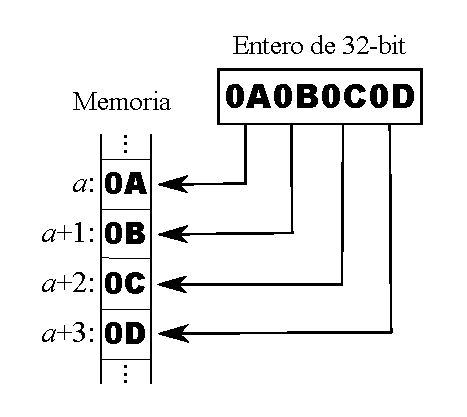
\includegraphics[width=\linewidth/3]{capitulo5/big_endian}
		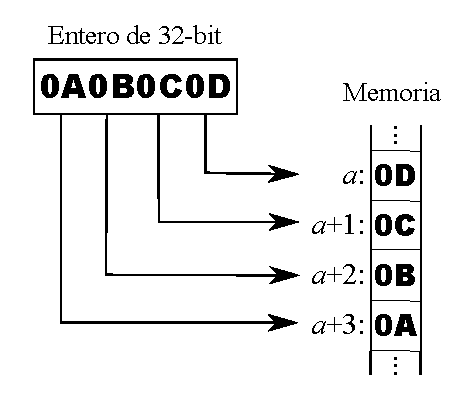
\includegraphics[width=\linewidth/3]{capitulo5/little_endian}
		\par\end{centering}
	\smallskip
	\caption[Big-endian y little-endian]{\label{fig:endianness} Big-endian (izquierda) y little-endian (derecha). \cite{wiki_endianness}}
\end{figure}
	
\smallskip

Por otro lado, también sabemos que ciertos valores, como el \textit{delta} de cada evento o el tamaño de datos de los meta-eventos, son de longitud variable: cada \textit{byte} tiene un significando de 7 \textit{bits}, los menos significativos. Mientras el último \textit{bit} sea 1, entonces el \textit{byte} siguiente del archivo corresponde, de igual forma, a otros 7 \textit{bits}, que se colocarían a la derecha (menos significativos).

\smallskip

\begin{figure}[H]
	\noindent \begin{centering}
		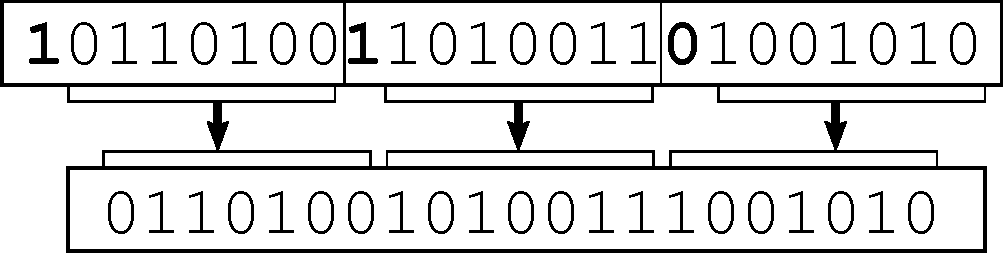
\includegraphics[width=\linewidth/2]{capitulo5/varlen}
		\par\end{centering}
	\smallskip
	\caption{\label{fig:varlen} Campo de longitud variable.}
\end{figure}

\smallskip

Además, podemos ver que todos los tipos de evento se numeran a partir de $80_{16}$, o sea, su \textit{bit} más significativo es 1. Si el analizador buscara un tipo de evento y encontrara un valor por debajo de este número, significa que el archivo está obviando el tipo de evento, y está indicando los parámetros ---cuyo tope es 127---.

\subsubsection{Prototipo}

En primer lugar hacemos una implementación sencilla en Python, que nos permita comprobar que hemos aplicado correctamente los conceptos.

Todos los valores de los tipos enumerados se hacen mediante constantes. Tal como dicta el diseño, la clase principal es \code{MidiFile}, que recibe un nombre de archivo. Los métodos se han implementado de la siguiente forma:

\begin{description}[style=nextline]
	\item[\code{\_\_init\_\_(self, pathname)}]
	Constructor: crea un archivo \acrshort{MIDI} completo desde un nombre de archivo (\code{pathname}). Abre el archivo, desempaqueta la cabecera y escribe los atributos del objeto en consecuencia. A continuación, inicializa la lista de pistas llamando al constructor de \code{MidiTrack} tantas veces como pistas indica el archivo.
	
	\item[\code{\_\_len\_\_(self)}]
	Devuelve el tamaño de la lista de pistas.
	
	\item[\code{\_\_getitem\_\_(self, key)}]
	Devuelve la pista indicada (\code{key}).
	
\end{description}

De esta forma, un archivo es sustancialmente una lista de pistas, y define los siguientes métodos:

\begin{description}[style=nextline]
	\item[\code{\_\_init\_\_(self, file)}]
	Constructor: crea una pista a partir de un fichero abierto (\code{file}), cuyo puntero debe estar al inicio de una nueva pista. Análogamente al constructor de \code{MidiFile}, analiza la cabecera, comprueba que sea válida y genera una lista de eventos utilizando para ello \code{MidiEvent.parseEvent()}
	
	\item[\code{\_\_iter\_\_(self)}]
	Permite iterar sobre los eventos la pista, devolviendo un iterador de la lista de eventos.	
\end{description}

Otra de las clases a implementar es \code{MidiEvent}, que representa cada uno de los eventos contenidos en un archivo, y contiene los siguientes métodos:

\begin{description}[style=nextline]
	\item[\code{\_\_init\_\_(self, delta, value, param1, param2)}]
	Constructor: crea un evento \acrshort{MIDI}, copiando en el sujeto (\code{self}) el retardo temporal (\code{delta}), el tipo de evento, junto al canal (\code{value}) y los parámetros (\code{param1} y \code{param2}).
	
	\item[\code{\_\_repr\_\_(self)}]
	Devuelve una cadena que expresa la representación del objeto, de la siguiente forma:
	
	\begin{center}
		<delta>: Event <tipo>@<canal> ( <Parámetro 1>, <Parámetro 2> )
	\end{center}
	
	\item[\code{note(self)}]
	Devuelve el código de nota (primer parámetro).
	
	\item[\code{velocity(self)}]
	Devuelve la intensidad sonora (primer parámetro).
	
	\item[\code{aftertouch(self)}]
	Devuelve la variación de intensidad, sita en el segundo parámetro si el tipo es \code{NOTE\_AFTERTOUCH} o en el primero en otro caso.
	
	\item[\code{controller(self)}]
	Devuelve el número de controlador (primer parámetro).
	
	\item[value\code{(self)}]
	Devuelve el valor del controlador (segundo parámetro).
	
	\item[program\code{(self)}]
	Devuelve el código de programa (primer parámetro).
	
	\item[pitch\code{(self)}]
	Devuelve el valor del \textit{pitch-bend} uniendo los parámetros:
	
	\begin{center}
		$p_1 \; | \; (p_2 << 7)$
	\end{center}
	
	\item[parseEvents(file)]
	Método de clase. Analiza todos los eventos de la pista actual en el archivo (\code{file}) hasta encontrar el meta-evento \code{END\_OF\_TRACK}. Su funcionamiento es el siguiente:
	
	\smallskip
	
	\begin{figure}[H]
		\noindent \begin{centering}
			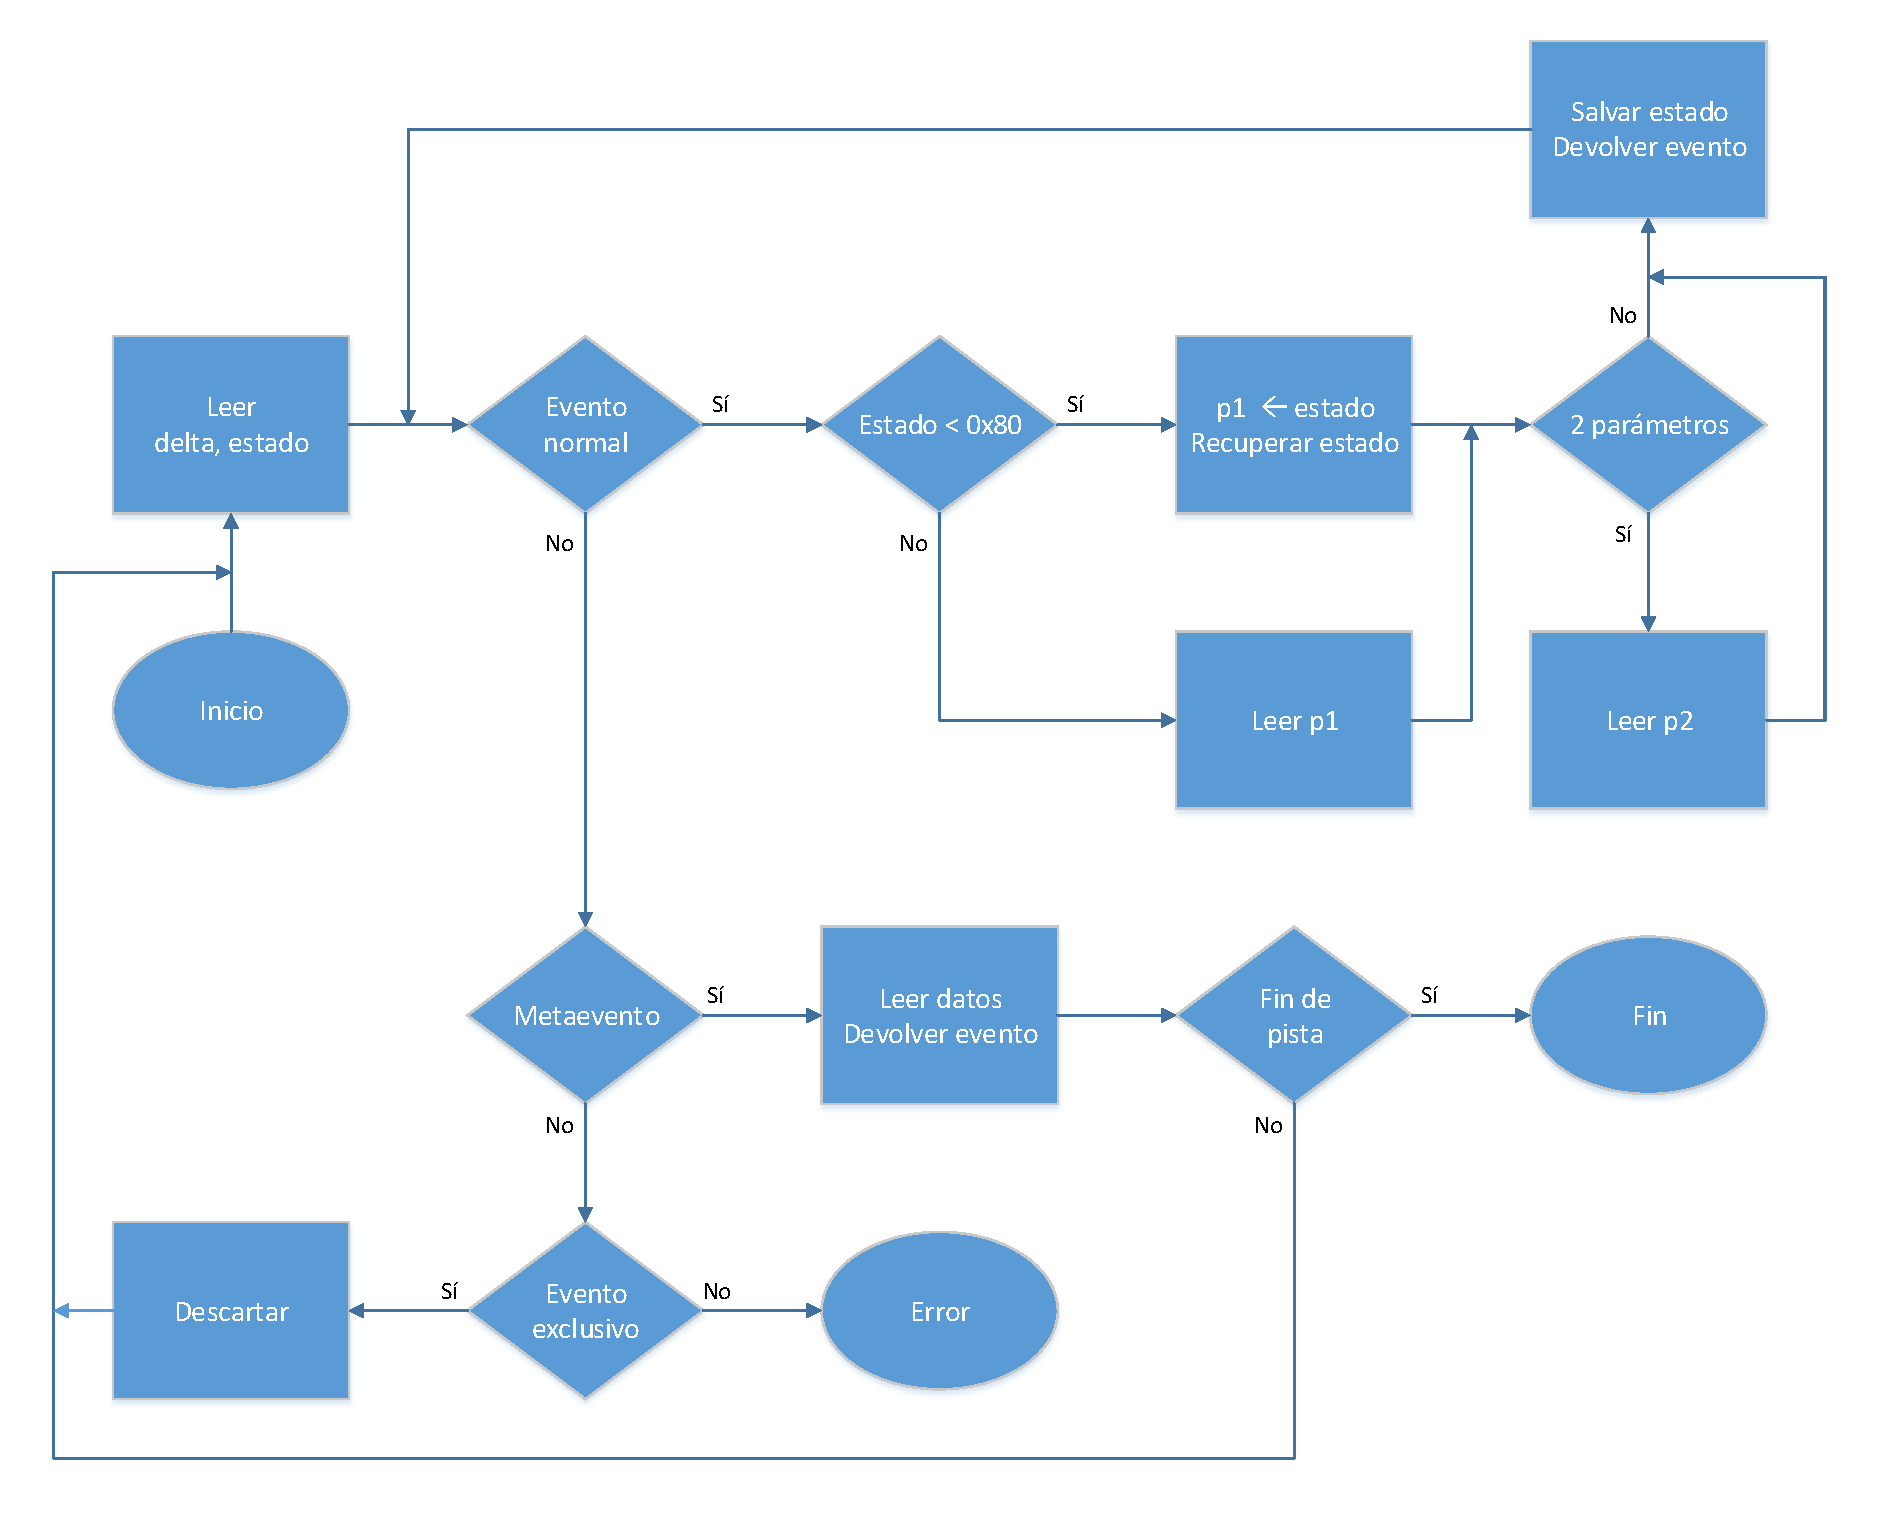
\includegraphics[width=\linewidth*2/3]{capitulo5/flujo_parser}
			\par\end{centering}
		\smallskip
		\caption{\label{fig:flujo_parser} Diagrama de flujo del analizador.}
	\end{figure}
	
	\smallskip
	
	\item[\code{varlen(file)}]
	Es una función auxiliar privada que recibe el archivo (\code{file}) apuntando a un campo de longitud variable (véase la figura \ref{fig:varlen}) y devuelve su valor.
	
\end{description}

Por último, la clase \code{MetaEvent} hereda de \code{MidiEvent} y, de acuerdo al diseño, tiene los siguientes métodos:

\begin{description}[style=nextline]
	\item[\code{\_\_init\_\_(self, delta, evtype, data)}]
	Constructor. Crea un metaevento copiando en el sujeto (\code{self}) el retardo temporal (\code{delta}), el tipo de meta-evento (\code{evtype}) y la cadena de datos (\code{data}).
	
	\item[\code{\_\_repr\_\_(self)}]
	Devuelve una cadena que expresa la representación del objeto, de la siguiente forma:
	
	\begin{center}
		<delta>: Meta-event <tipo>@<canal> ( <Parámetro 1>, <Parámetro 2> )
	\end{center}
	
	\item[\code{number(self)}]
	Devuelve el número de secuencia (primer \textit{byte} de la cadena).
	
	\item[\code{text(self)}]
	Devuelve la propia cadena de texto.
	
	\item[\code{channel(self)}]
	Devuelve el canal por defecto (primer \textit{byte} de la cadena).
	
	\item[\code{tempo(self)}]
	Calcula el \textit{tempo} en \textit{$\mu s / \quarternote$}. Este valor ocupa 3 \textit{bytes}, que se acuñan así:
	
	\begin{center}
		($d_0 << 16) \; | \; (d_1 << 8) \; | \; d_2$
	\end{center}
	
	\item[\code{offset(self)}]
	Devuelve el desplazamiento temporal en una lista con el siguiente contenido:
	
	\begin{enumerate}
		\item Velocidad, según los 2 \textit{bits} más significativos del primer \textit{byte} de la cadena:
		
		\begin{itemize}
			\item $d_0[7:6] = 0 \Rightarrow 24 \; fps$
			\item $d_0[7:6] = 1 \Rightarrow 25 \; fps$
			\item $d_0[7:6] = 2 \Rightarrow 30 \; fps$
		\end{itemize}
		
		\item Número de horas ($d_0[5:0]$).
		\item Número de minutos ($d_1$).
		\item Número de segundos ($d_2$).
		\item Número de cuadros ($d_3$).
	\end{enumerate}
	
	\item[\code{time(self)}]
	Devuelve la marca de compás en una lista, de la siguiente forma:
	
	\begin{enumerate}
		\item Numerador: $d_0$.
		\item Denominador: $2^{d_1}$.
		\item Número de \textit{ticks} entre cada marca del metrónomo: $d_2$.
		\item Subdivisión, en \textit{fusas / click}: $d_3$.
	\end{enumerate}
	
	\item[\code{key(self)}]
	Devuelve la tonalidad en una lista, con los siguientes valores:
	
	\begin{enumerate}
		\item Número de $\sharp$ si es positivo, o número de $\flat$ si es negativo: $d_0$.
		\item Modo: $d_1$
	\end{enumerate}
\end{description}

Ya que es una prueba de concepto, el analizador emitirá un \textit{log} con  todos los datos extraídos de un archivo. Un ejemplo de salida es el siguiente:

\smallskip

\begin{figure}[H]
	\noindent \begin{centering}
		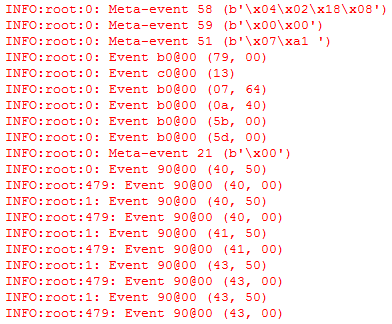
\includegraphics[width=\linewidth/2]{capitulo5/cap_parser}
		\par\end{centering}
	\smallskip
	\caption{\label{fig:cap_parser} Salida del prototipo del analizador.}
\end{figure}

\smallskip

\subsubsection{Implementación final}

Una vez puesto a prueba el analizador de \acrshort{MIDI} en Python, lo pasamos a C. Al ser un lenguaje no orientado a objetos, hay que introducir algunos cambios, pero el algoritmo es el mismo que el del prototipo. Sin embargo, las funciones no diferirán mucho del lenguaje anterior, porque en Python hay que poner el sujeto del método como primer parámetro, y en la nueva implementación haremos lo mismo. La diferencia más significativa es que tendremos que insertar un \textbf{destructor}.

En primer lugar, definimos los \textbf{tipos enumerados}:

\begin{description}
	\item[\code{enum format\_t}] Formato del archivo:
	
	\begin{description}
		\item[\code{SINGLE\_TRACK}] Una sola pista.
		\item[\code{MULTIPLE\_INDEPENDENT}] Varias pistas, simultáneas.
		\item[\code{MULTIPLE\_SIMULTANEOUS}] Varias pistas, independientes.
	\end{description}
	
	\item[\code{enum division\_t}] Unidad de medida de la división de tiempo:
	
	\begin{description}
		\item[TICKS\ PER\ BEAT] La división se especifica en \textit{ticks}/\quarternote.
		\item[FRAMES\_PER\_SECOND] La división se especifica en \textit{ticks/fotograma}.
	\end{description}
	
	\item[\code{enum midievent\_type\_t}] Tipo de evento \acrshort{MIDI}. Se enumeran en la tabla \ref{tab:midi_eventos}.
	\item[\code{enum metaevent\_type\_t}] Tipo de meta-evento. Se enumeran en la tabla \ref{tab:midi_metaeventos}.
	
	\item[\code{enum midimode\_t}] Modo tonal:
	
	\begin{description}
		\item[MAJOR] Modo mayor.
		\item[MINOR] Modo menor.
	\end{description}
\end{description}

Aparte del resto de transformaciones obvias, en pro de la velocidad de ejecución, hacemos los siguientes cambios:

\begin{enumerate}
	\item Anteponemos un \textbf{prefijo} a las funciones propias de cada estructura. El primer parámetro de todas ellas será un puntero a la misma.
	
	\item Eliminamos las funciones de consula que acceden llanamente a los parámetros, y a cambio sustituimos los parámetros simples por \textbf{uniones} con los nombres de las funciones.
	
	\item Ya que no podemos conocer a \textit{priori} el número de eventos que contendrá una pista, vamos a interpretar la composición propuesta por el diagrama \ref{fig:uml_midi} como una \textbf{lista enlazada} de eventos. Ya que la inserción y la lectura van a ser secuenciales, garantizamos una eficiencia algorítmica $O(1)$ en cada acceso.
\end{enumerate}

\subsection{Planificador}

\subsubsection{Prototipo}

\subsubsection{Implementación}

\subsubsection{Concurrencia}

\subsection{Salida GPIO}

\subsubsection{Prototipo}

\subsubsection{Implementación}

\subsubsection{Acceso directo al GPIO}

\subsubsection{Mapeo y tolerancia}

\subsection{Demonio}

\subsubsection{Características}
\subsubsection{Script de arranque}
\subsubsection{Permisos de usuario}

\subsection{Servidor socket}

\subsection{Servidor UART}

\subsection{Modo Ingeniería}

\subsubsection{Control de salida}
\subsubsection{Control de entrada}
\subsubsection{Máquina de estados}

\subsection{Seguridad}
\subsubsection{Permisos de usuario}
\subsubsection{Conexiones simultáneas}
\subsubsection{Compatibilidad con MIDI estándar}

\subsection{Código de preinstalación}

\section{Interfaz web}

\subsection{Estructura principal}
\subsubsection{Plantillas}
\subsubsection{Controlador}
\subsubsection{Sesión}

\subsection{Traductor}

\subsection{Control de energía}

\subsection{Portada}
\subsubsection{Autentificación}

\subsection{Navegación}

\subsection{Conexión a la base de datos}

\subsection{Conexión al demonio}
\subsubsection{Prototipo}
\subsubsection{Implementación}

\subsection{Reproductor}
\subsubsection{Vista}
\subsubsection{Controlador}

\subsection{Gestión de listas y piezas}
\subsubsection{Vista}
\subsubsection{Controlador}

\subsection{Asignación del mando}
\subsubsection{Vista}
\subsubsection{Controlador}

\subsection{Seguridad}
\subsubsection{Inyección de código SQL}
\subsubsection{Inyección de código shell}
\subsubsection{Permisos de superusuario}


\section{Base de datos}

\section{Aplicaciones auxiliares}
\subsection{Información de archivo MIDI}
\subsection{Simulador de reproducción}
\subsection{Terminal del reproductor}
\subsection{Comprobación de contraseña}
\subsection{Instalador del servidor}